\documentclass[12pt,letterpaper,onecolumn]{article}
\usepackage[latin1]{inputenc}
\usepackage{amsmath}
\usepackage{amsfonts}
\usepackage{amssymb}
\usepackage{graphicx}
\linespread{1.6}
\usepackage[margin=0.8in]{geometry}
\usepackage{fancyhdr}
\pagestyle{fancy}
\author{Devin White}
\title{Dynamic Task Allocation For Multi-Agent Systems Utilizing Hierarchical Task Delegation}
\lhead{}
\rhead{Devin White}
\begin{document}
	\begin{titlepage}
		\maketitle
	\end{titlepage}
	\begin{titlepage}
		\tableofcontents
	\end{titlepage}
	\section{Abstract}
	This paper covers what defines a multi agent system and what dynamic task allocation is in the context of such a system. It then goes to contrast several opposing implementation choices when designing a task allocation system. Choices such as centralized versus distributed, as well as allowing agents to communicate globally or locally, must be selected. After, several approaches to dynamic task allocation proposed by various researchers are examined. From these methods I derive a new implementation for dynamic task allocation, designated as a hierarchical task delegation model for dynamic task allocation in multi agent systems. Finally, I will outline the implementation for the model, examine the benefits this system provides in terms of communication costs, and note some future improvements to this task allocation technique.
	\section{Multi Agent Systems and Task Allocation}
	\subsection{Defining A Multi Agent System}
	A Multi Agent System (MAS) is a pattern of information and control / collaboration relationships among agents, as well as the distribution of problem solving capabilities amongst them. [Weiming Shen, et al. 2001] An agent in such a system is composed of a set of skills or resources available to it and a representation of what it can do, so that other agents may call upon that agent, and so that it can reason about whether or not it can complete a requested task. [Weiming Shen, et al. 2001] A MAS structure gives a high level view of how a group of agents solves problems and what role each agent plays in some organized manner. [Weiming Shen, et al. 2001] Mallone proposed that such an organization consists of a group of agents, the set of activities those agents can perform, a set of connections between agents, and a set of goals or evaluation criteria by which the combined activities of the agents are calculated. [Weiming Shen, et al. 2001]
	\subsection{Defining Dynamic Task Allocation in a MAS}
	Dynamic task allocation in a MAS is simply described as  a situation where an agent has a task that it cannot complete on its own. [Dayong Ye, et al. 2009] It therefore must discover other agents which contain the appropriate resources or skills, and delegate all or part of that task to them. [Dayong Ye, et al. 2009] An optimal dynamic task allocation system will allocate tasks amongst the agents in a way that maximizes the number of successfully completed tasks and overall system utility. [Singhal, V., Dahiya, D., 2015] This optimal allocation should improve the overall performance of the MAS, lower overall execution time, reduce costs incurred for each task allocation, and minimize the communications between agents. [Singhal, V., Dahiya, D., 2015] To do this requires collaboration between agents, which takes place through communication and coordination of plans and actions among agents within the system. [Weiming Shen, et al. 2001] Many different approaches have been taken to address the complex task of getting agents to coordinate for efficient task allocation. [Singhal, V., Dahiya, D., 2015] They each use differing methods to achieve their implementation regarding communication and coordination. The next section will cover several of these implementation choices.
	\section{Comparison of Task Allocation Structures}
	\subsection{Centralized versus Distributed}
	A centralized model for task allocation involves using a central controller with a global view of the environment to allocate tasks. [Dayong Ye, et al. 2009] Opposite that, there is fully decentralized distributed control, such as the greedy distributed allocation protocol (GDAP), which only allows agents to communicate between directly linked neighbors. [Dayong Ye, et al. 2009] Centralized control benefits from its global awareness, allowing it to make more informed decisions when allocating tasks. [Dayong Ye, et al. 2009] However, this also means the whole system relies on the central controller functioning properly. [Dayong Ye, et al. 2009] This single point of failure results in decreasing robustness of the system. [Singhal, V., Dahiya, D., 2015] Additionally, as the system scales up, the centralized controller can be overloaded with information, drastically increasing the time required to allocate tasks. [Dayong Ye, et al. 2009] A fully distributive approach allows a task to arrive at any agent, improving robustness of the system compared to a centralized approach. [Singhal, V., Dahiya, D., 2015] This approach is also significantly more scalable, as any one agent has access to only its direct neighbors. [Dayong Ye, et al. 2009] On the other hand, as it scales, the total number of communications between agents increases, as agents must communicate through their neighbors, which makes the cost of communication significantly higher. [Dayong Ye, et al. 2009] Task allocation may fail due to the sheer amount of time taken when communicating over many neighbors. [Dayong Ye, et al. 2009] A combination of these two approaches relies on a shallow hierarchical structure, where some agents act as mediators that have connections to some subset of the total collection of agents. [Dayong Ye, et al. 2009] This removes the need for a single centralized dispatcher, and reduces the significant increase of communications created when only associating with neighbors. 
	\subsection{Local versus Global}
	Once it is determined which agents will be given the tasks to allocate, the next major design choice is how locally or globally tasks may be allocated. As stated above, systems which have a global scope for communication face the issue of making the allocator of a task access too many agents when making their allocation decision. Similarly, limiting the scope down to neighbor agents increases the number of communications significantly when the task cannot be allocated locally. An ideal scope is a group one, where agents are grouped together and communication between groups is handled via a facilitator agent. [Weiming Shen, et al. 2001] A facilitator provides the message-passing and routing required to  obtain knowledge about its group members, and determine which tasks to allocate, and to whom. [Weiming Shen, et al. 2001] This structure of facilitators reduces communications by restricting each agent's knowledge of other agents based on their group, and scales the points of failure to the number of facilitators in the system. [Weiming Shen, et al. 2001] This group approach can also be extended to a community approach where agents can belong to multiple communities, each with an initiator agent (acting as a local facilitator) that allocates tasks, where agent cooperation is constrained to a community. [Wanyuan Wang, Yichuan Jiang, 2014] A community would be a collection of related units, ideally related spatially or due to being able to meet a given tasks' resource requirements. [Wanyuan Wang, Yichuan Jiang, 2014] The hierarchical task delegation system described in this paper is modeled after a combination of facilitator and community relationships.
	\subsection{Hierarchical versus Horizontal}
	After examining centralized versus distributed, and local versus global task allocation techniques, I have come to the conclusion that a well designed and efficient MAS must strike a balance between these opposing architectures. The MAS must allow the work of allocating tasks to be spread out over multiple agents for increased system robustness, but also maintain restrictions on communication to groups or communities of agents so that communication costs remain manageable for larger systems. 
	The next issue then, is how to manage these groups of agents, either in a more structured, hierarchical manner, or in a more horizontal or peer to peer approach. A hierarchical structure is composed of some form of tree of agents in parent-child relationships. [Farazmand, E., et. al., 2005] The network of agents is composed of managers and individuals, with an individual being on a leaf node of the hierarchy. [Urakawa, K., Sugawara, T., 2013] These individuals possess resources needed to complete given tasks, and managers play the role of allocating tasks or subtasks to their children, from a root manager down to an individual. [Urakawa, K., Sugawara, T., 2013] At any level of the hierarchy, agents can communicate with adjacent agents, those being their parents or children, restricting overall communications. [Urakawa, K., Sugawara, T., 2013] A horizontal or peer to peer approach also allows communication with adjacent agents, however these neighbors do not exhibit parent-child relations on other agents. [Farazmand, E., et. al., 2005] Communities of neighbors can be formed that restrict agent communications, with each community having an initiator that receives a task to allocate to its group or neighbors. [Wanyuan Wang, Yichuan Jiang, 2014] Cooperation is restricted to intra-community members, with the initiator negotiating amongst member agents to successfully allocate a task. [Wanyuan Wang, Yichuan Jiang, 2014] Both the hierarchical and horizontal models attempt to restrict the scope of individual agents, thereby reducing the total number of communications in the system. However, a purely hierarchical approach ignores the need for communications between agents at a given hierarchy level, instead only allowing parent-child interactions. Opposite that, the community approach restricts itself to its own subset of agents, allowing full communication between members, but does not have the depth a hierarchy creates, limiting the possibilities of combinations of agents to the group members. Therefore I propose a hierarchical task delegation model, which attempts to bring a hierarchical structure to the community model, essentially creating a hierarchy of communities.
	\section{A Hierarchical Task Delegation Model}
	\subsection{Outline of the HTD Model}
	I refer to my system for dynamic task allocation in a MAS as the hierarchical task delegation (HTD) model. This is due to the hierarchical structure of the agents, and the idea that an agent 'delegates' tasks to other agents lower in the hierarchy. The hierarchy is composed of director agents and worker agents, with worker agents being at the bottom level of the hierarchy. Worker agents hold all of the resources in the system, with director agents having no actual resources. HTD can be broken down into three parts: task procurement, task delegation, and task commitment. Task procurement is when an agent receives a set of tasks, and, if the current agent has enough resources at their disposal to complete the given task, places that task into a priority queue ordered by profitability. Task delegation is the process of attempting to delegate each task to the collection of child agents the receiving agent is responsible for. This can either be to a single agent, or, if no single child agent has the required resources, to a coalition of agents. The agent or agents are selected based on how 'fit' that agent or coalition of agents are for the task. Task commitment is a confirmation sent by the worker agents at the bottom of the hierarchy after they have been delegated a task. At this point, worker agents who have accepted a task can form a coalition, and commence with task execution.
	\subsection{Influences}
	\subsubsection{Extended Task Allocation Method with Link Generation and Elimination (eTALGE)}
	The HTD model was heavily influenced from the model proposed by Kazuki Urakawa and Toshiharu Sugawara. Their model was based on a hierarchical approach, providing efficiency for decision making, and established on the fact that actual nodes in large-scale systems often form tree overlay networks. [Urakawa, K., Sugawara, T., 2013] They used a hierarchy consisting of two types of agents, managers and individuals. Managers branch out from the root manager, and select subtasks of a given task to allocate to its children. Individuals are the leaf nodes, and are responsible for allocating resources to tasks. Each node can only communicate with its parent and its children. This structure limits and reduces total communications in the system. [Urakawa, K., Sugawara, T., 2013]
	\subsubsection{Community Aware Social Networked Multi Agent System (CS-SN-MAS)}
	My HTD approach also takes from the social networked MAS considered by Wanyuan Wang and Yichuan Jiang. They introduce a model made up of communities, each consisting of a subset of the total population of agents, where intra-community communication is much greater than inter-community communication. Some agents can exist in more than one community, and in this way create overlapping communities. An initiator agent within a community receives a task, and then negotiates with the community members to allocate the task in a way that satisfies a community consensus. There are two key formulas taken from this system which I will use in my HDT model:
	\begin{itemize}
		\item Task Profitability: Let W(t) be the sum of resources required for a task t, let p(t), be the payment from completing t, then profitability(t) = p(t) / W(t) [Wanyuan Wang, Yichuan Jiang, 2014]
		\item Task Fitness: Let ar(t) be the sum of a group of agents resources, let req(t) be the sum of required resources to complete a task, then $fitness(t) = 1 - \dfrac{\sum_{i=1}^{k} max(ar(t, r_{i}) - req(t, r_{i}), 0)}{\sum_{i=1}^{k} ar(t, r_{i})} $ [Wanyuan Wang, Yichuan Jiang, 2014]
	\end{itemize}
	\subsubsection{Efficient Task Allocation Protocol (ETAP)}
	I will also reference work done by Dayong Ye and Zhiqi Shen. Their solution to task allocation is for a P2P MAS. It is essentially a more restricted version of the community model, allowing the initiator to talk exclusively to its neighbors. If within that set of agents there are no further resources to complete the current task, it divides up the remaining tasks amongst the neighbors, and they in turn attempt to allocate the tasks to their neighbors, making them mediators for a given subset of the remaining tasks. I look to adapt their method of dividing up tasks to a more hierarchical method. 
	\subsection{Assumptions}
	There are a few assumptions to be made when examining the proposed hierarchical task delegation method. Firstly, I assume there is a static number of agents within the system, as accounting for changes in the hierarchy would not be categorized under task allocation. Next, I assume any given director of a group of agents maintains the total amount of resources of all agents in the group. Since the system has a static number of agents, and an already established hierarchy, high level directors will have already consulted lower members to determine what resources they have. Finally, this system uses the assumption that agents within a group are clustered near each other spatially, and therefore it is preferential that worker agents in a group work together over agents from another group.
	\subsection{Implementation of the HTD Model}
	\subsubsection{Definitions}
	\begin{enumerate}
		\item A Hierarchical Task Delegation model for a MAS is defined as $ HTD = <A, F, G> $ where $A = \{a_{1}, a_{2},\dots, a_{m}\}$ is the set of agents in the system, $F = \{(a_{1}, f(a_{1})), \dots, (a_{m}, f(a_{m}))\} $ is the set of agent-facilitator relationships, and $ G = \{(a_{1}, G_{1}), (a_{2}, G_{2}), \dots, (a_{m}, G_{m})\} $ is the set of facilitator-group relationships.
		
		\item An agent $a_{i} = \{f(a_{i}), R_{i}, G_{i}\} $ where $f(a_{i})$ is the facilitator of the agent, $ R_{i}$ is the set of resources owned by the agent, and $ G_{i}$ is the group of agents this agent facilitates.
		
		\item Given a set of tasks $T = \{t_{1}, t_{2}, \dots, t_{n}\} $, $t_{j} = \{R_{j}, p(t_{j}), ini(t_{j}), TTL(t_{j})\}$ where $R_{j}$ is the set of resources required to complete $t_{j}$, $p(t_{j})$ is the payoff from completing $t_{j}$, $ini(t_{j})$ is the initiator of $t_{j}$, which will await a response from agents it sent tasks to, and $ TTL(t_{j})$, which is the Time To Live for the task. TTL will help to restrict selecting agents from many different branches of the hierarchy.
		
		\item A contract $c_{s} = \{task(c_{s}), R_{s}\}$, where $task(c_{s})$ is the task associated with the contract, and $R_{s}$ is the number of resources required for the contracts' fulfillment
	\end{enumerate}
	
	\subsubsection{Model Structure}
	\begin{figure}
		\centerline{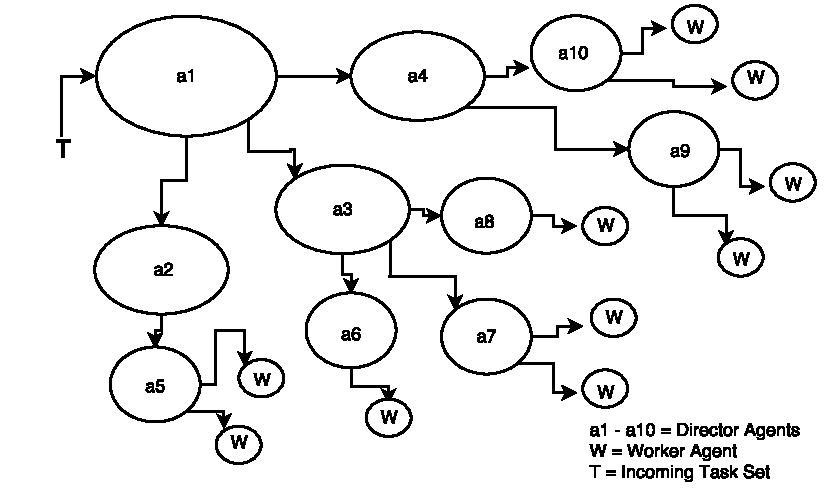
\includegraphics{HTDModel.pdf}}
		\caption{Relationships between agents in the HTD Model}
	\end{figure}
	As stated in Definition 1, the Hierarchical Task Delegation structure is composed of a graph of agents and their relationships. These relationships form a hierarchy composed of L+1 levels, where there are L levels of directors, and one level of workers at the base. Director agents have one or more connections to the group of agents they direct, and store the sum of all resources of agents within that group. Worker agents have no connections to a group, but have access to the actual resources of the system, and therefore handle the actual task execution. It is the job of directors to 'delegate' tasks down the hierarchy to achieve the 'best fitting' collection of worker agents. The best fit set of worker agents is defined as:
	\begin{itemize}
		\item Agents that are spatially close, and then agents that have the best fit regarding the resource requirements $fitness(t) = 1 - \dfrac{\sum_{i=1}^{k} max(ar(t, r_{i}) - req(t, r_{i}), 0)}{\sum_{i=1}^{k} ar(t, r_{i})} $ [Wanyuan Wang, Yichuan Jiang, 2014]
	\end{itemize}
	It is important to note my assumption that agents in the same hierarchy group are spatially close to each other, because this means it will take less time once the task is delegated to worker agents for those agents to form a coalition and execute the task than if agents from another branch of the hierarchy were required. Therefore HTD will always select agents from the same group first in an attempt to minimize time expended during task commitment.
	
	\subsubsection{Dynamic Task Allocation}
	\paragraph{Task Procurement}
	Dynamic task allocation using HTD begins by task procurement, having some agent in the system receive a task t or set of tasks T. Any agent is able to handle this process of receiving tasks, however it is more likely that agents further up the hierarchy will be queried due to the fact that they have more resources available to them, and will be able to handle more tasks. This means higher level director agents are much more likely to obtain task requests. Once a task or tasks have been obtained by a receiver agent, they will rank each task based on its profitability ($ profit(t_{i}) = p(t_{i}) / \sum_{j=1}^{k}R^{t_{i}}_{j}$), the payoff over the sum of resources. Then, each task will be examined in order of rank, and an attempt to delegate the task to the local group will begin. If at any point the receiver determines they do not have enough resources to complete the current task, they will respond to the initiator of the task with a failed to allocate message. 
	\paragraph{Task Delegation}
	The next phase, task delegation, requires the current agent to determine who to delegate the currently highest ranked task to. If the current agent is a worker agent, then there is no other agent to delegate to, so the agent will accept the task. If the agent is a director agent, it has other agents which  it can delegate the task to, so it will attempt one of two cases in order:
	\begin{description}
		\item[Case 1] There is an agent with the resources to complete the task in the current agents' group. If this is the case, then rank the agents by fitness to the task (formula above) and create a contract equivalent to the resource requirements of the task to delegate to the most fit agent.
		\item[Case 2] There is no individual agent in the group with the resources to complete the task. Then generate all possible coalitions of agents with the resources to complete the task, and rank those coalitions by fitness. Select the most fit coalition, and divide the task into contracts. Each contract is for the current task, and its R is equal to a portion of the required resources for the task. Coalition sizes must be $>=2$, since case 1 proved no one agent could complete the task. The contracts will be assigned to each agent in the coalition in order of their available resources. Coalition member $member_{1}$ would obtain a contract for all of its unallocated resources ($c_{1} = \{t_{i}, R_{member_{1}}\}$), and $member_{n}$ would obtain a contract for any remaining required resources ($cn = \{t_{i}, R_{t_{i}} - (\sum_{k=1}^{n-1} R_{c_{k}})\}$). The agent then delegates each contract to the respective coalition member.
	\end{description}
	The process of delegating and creating contracts will repeat itself through the hierarchy until it reaches a worker agent, at which point that agent accepts the contract, thereby assigning itself to the task.
	\paragraph{Task Commitment}
	The final phase of HTD is task commitment. This is the point immediately after a contract is received by a worker agent. When the worker agent accepts the contract, it assigns itself to that task, sending a confirmation for the contract to their director. The director will wait for all group members it has issued a contract to to send a confirmation, then it will send a confirmation to its director, and so on, back up to the original task contract. Once the original task receiver obtains confirmations from the agents it issued contracts to, it sends a confirmation back through the hierarchy, where it will reach all worker agents assigned to the task. The workers will then lock in to their task, not accepting any new requests. The director tree is updated to reflect the now allocated agents, and fitness calculations have the resources from currently allocated tasks decremented from their total resources. The worker agents then assemble into a coalition of agents to execute the task. Workers will respond with a completed or failed message to their directors after attempting execution of the task. This will update the hierarchy, unlocking the workers from their previous task, and removing that task from each involved director. Eventually, this will propagate back to to initiator of the task, and that agent will send a message containing the result of the task to the original task issuer.
	
	\paragraph{Allocation Constraints}
	The whole task allocation process of procurement, delegation, and commitment must be completed within the task's Time To Live (TTL). This makes sure that at any step the system is not trapped waiting for a response from an agent, and also restricts how far contracts can be sent breadth-wise in the hierarchy. With the assumption that groups of agents are 'closer' to each other, spreading contracts amongst many group  members at a high level in the hierarchy could potentially create a coalition of worker agents that are far from each other. The TTL will make sure time between requests is not exceeded.
	
	\subsection{Analysis of the HTD Model}
	Hierarchical Task Delegation should improve overall system robustness over a centralized implementation while simultaneously reducing the number of communications within the system compared to a horizontal approach. Any agent can receive tasks, but I assume tasks will enter on a higher level of the hierarchy. This means there will always be some delegation and commitment communication costs. The total amount of communications in the system is delegation cost(d) + commitment cost(c).
	\paragraph{Best Case}
	The best scenario is one where the given task requires only one worker to complete. Then communication costs are: $cost = 2(d + c) = 2(|G_{initiator(t_{i})}| + |G_{selected_{1}}| + \dots + |G_{selected_{n}}|) + (L+1))$, where $|G_{initiator(t_{i})}|$ is the cardinality of the group directed by the initiator, each subsequent term being the cardinality of the group of the agent the task was delegated to, and L+1 is the depth of the hierarchy.
	\paragraph{Worst Case}
	The worst scenario is if a task requires all available workers in the system where the initiator of the task is within their director hierarchy. For that situation, communication costs are: $cost = 4(|G_{initiator(t_{i})}| + \sum|G_{ar}| + \sum|G_{ar_{r}}| + \dots)$ where $|G_{initiator(t_{i})}|$ is the cardinality of the group directed by the initiator, $\sum|G_{ar}|$ is the summation of the cardinalities of the groups of agents where $F(ar, f(initiator(t_{i})))$, and $\sum|G_{ar_{r}}|$ is the summation of the cardinalities of the groups of agents where $F(ar_{r}, f(ar))$, continuing until reaching the summation of the number of agents in all groups under the initiator. There are four messages sent to each agent under the initiator, request for resources, contract delegation, commitment response, and confirmation response. Unless the system is small, or the initiator is low in the hierarchy, the TTL for a task should cause a failure before reaching every agent under the initiator.
	\paragraph{Average Case}
	When the system has not yet allocated any tasks, there will be an abundance of available resources. This means that allocations should be fast, as needed resources can be accessed without entering multiple sections of the hierarchy. As tasks are allocated, the performance will degrade, and searching for workers with the required resources demands exploring a larger number of branches within the system.
	\subsection{Improvements}
	There are two major improvements I am interested in making to the HTD system, namely including distance to the task in allocation calculations, and implementing learning algorithms.
	\paragraph{Allocation Including Distance}
	Distance is an important metric currently overlooked in the HTD approach. Task allocation is already done based on the assumption that agents within groups in the hierarchy are spatially closer, but this could also include their distance from the given task. Incorporating distance from the task into the fitness metric would make sure that a task can be commenced faster, and improve the selection of worker agents for a given task.
	\paragraph{Delegation With Learning}
	The eTALGE system proposed by Kazuki Urakawa and Toshiharu Sugawara features learning that I believe would improve the flexibility and speed of the HTD model. They use an allocation policy that is learned through experience with a modified form of Q-learning, calculating the reward for when a team is successfully formed while not using Q values of the next step. [Urakawa, K., Sugawara, T., 2013] They also handle director task delegation through learning. The eTALGE model lets each director estimate what resources their subordinates have available based on their responses to delegated tasks. Each director can then adjust their delegation process based on these responses. 
	\section{Conclusion}
	In this paper, I looked at what is required for efficient dynamic task allocation in a MAS. I examined several implementation decisions, and determined that the best solution to dynamic task allocation in a MAS requires a balanced approach. Balance refers to spreading control out amongst director agents, and maintaining restricted communication over a structured framework. I then proposed my own model built from these concepts, hierarchical task delegation. Finally I outlined the assumptions, implementation, and communication costs of HTD, and looked at improvements that could augment this system in the future. To summarize, dynamic task allocation in a MAS is a complex problem with many possible combinations of techniques. However, favorable solutions are ones which strike a balance between implementation factors, and model real world interactions. 
	\section{References}
	\begin{enumerate}
		\item[][Weiming Shen, et al. 2001] Weiming Shen, Douglas H. Norrie and Jean-Paul A. Barthes, Multi-Agent Systems For Concurrent Intelligent Design and Manufacturing?, p.30-145, Published by Taylor and Francis, 11 New Fetter Lane, London EC4P 4EE,  2001.
		\item[][Dayong Ye, et al. 2009] Dayong Ye; Quan Bai; Minjie Zhang; Khin Than Win; Zhiqi Shen, "An Efficient Task Allocation Protocol for P2P Multi-agent Systems," in Parallel and Distributed Processing with Applications, 2009 IEEE International Symposium on , vol., no., pp.11-18, 10-12 Aug. 2009
		\item[][Singhal, V., Dahiya, D., 2015] Singhal, V.; Dahiya, D., "Distributed task allocation in dynamic multi-agent system," in Computing, Communication and Automation (ICCCA), 2015 International Conference on , vol., no., pp.643-648, 15-16 May 2015
		\item[] [Wanyuan Wang, Yichuan Jiang, 2014] Wanyuan Wang; Yichuan Jiang, "Community-Aware Task Allocation for Social Networked Multiagent Systems," in Cybernetics, IEEE Transactions on , vol.44, no.9, pp.1529-1543, Sept. 2014
		\item[] [Urakawa, K., Sugawara, T., 2013] Urakawa, K.; Sugawara, T., "Task allocation method combining reorganization of agent networks and resource estimation in unknown environments," in Innovative Computing Technology (INTECH), 2013 Third International Conference on , vol., no., pp.383-388, 29-31 Aug. 2013
		\item[] [Farazmand, E., et. al., 2005] Farazmand, E.; Shokoufi, A.; Lucas, C.; Habibipour, F., "Using a learning mechanism in matchmaking process of agents' negotiation in multi-agent systems," in Advanced Information Networking and Applications, 2005. AINA 2005. 19th International Conference on , vol.1, no., pp.59-64 vol.1, 28-30 March 2005
	\end{enumerate}
\end{document}
